% This is based on the LLNCS.DEM the demonstration file of
% the LaTeX macro package from Springer-Verlag
% for Lecture Notes in Computer Science,
% version 2.4 for LaTeX2e as of 16. April 2010
%
% See http://www.springer.com/computer/lncs/lncs+authors?SGWID=0-40209-0-0-0
% for the full guidelines.
%
%
%     To submit at Alberto Mendelzon Workshop 2018
%
%
\documentclass{llncs}

\hyphenation{do-cu-ment do-cu-ments}

\usepackage[utf8]{inputenc}

\usepackage{graphicx}
\usepackage{comment}
\usepackage[usenames, dvipsnames]{xcolor}
\definecolor{igual}{rgb}{0.21, 0.11, 0} 
\usepackage{hyperref}
\definecolor{dark-blue}{rgb}{0.0,0.0,0.1}
\definecolor{dark-green}{rgb}{0.0,0.1,0.0}
\definecolor{dark-red}{rgb}{0.1,0.0,0.0}
\hypersetup{
    colorlinks, linkcolor={dark-red},
    citecolor={dark-green}, urlcolor={dark-blue},
    pdftitle={What should Entity Linking link?},    % title
    pdfauthor={Henry Rosales-Méndez, Barbara Poblete and Aidan Hogan},     % author
    pdfsubject={LD4IE 2017},   % subject of the document
    pdfkeywords={multilingual;} {entity linking;} {information extraction;}, % list of keywords
}
\usepackage{amsmath}
\newcommand{\argmin}{\arg\!\min}
\newcommand{\argmax}{\arg\!\max}

%para el simbolo de chequeado
\usepackage{amssymb}% http://ctan.org/pkg/amssymb
\usepackage{pifont}% http://ctan.org/pkg/pifont
\newcommand{\cmark}{\ding{51}}%
%\newcommand{\xmark}{\ding{55}}%
\newcommand{\xmark}{}%

\usepackage{moreverb}% usar verbatim + box
\usepackage{breqn}

\usepackage{booktabs}

\begin{document}

\title{What should Entity Linking link?}
%
%
\author{Henry Rosales-M\'endez, Barbara Poblete and Aidan Hogan}
%
\authorrunning{Rosales-Méndez et al.} % abbreviated author list (for running head)
%
%%%% list of authors for the TOC (use if author list has to be modified)
%\tocauthor{Ivar Ekeland, Roger Temam, Jeffrey Dean, David Grove,
%Craig Chambers, Kim B. Bruce, and Elisa Bertino}
%
\institute{Center for Semantic Web Research, DCC, University of Chile \\
\texttt{\{hrosales,bpoblete,ahogan\}@dcc.uchile.cl}}

\maketitle              % typeset the title of the contribution
\begin{abstract}
Some decades have passed since the concept of named entity was used for the first time. From there, new lines of research have emerged in this environment, such as linking the entity mentions in a text collection with its corresponding knowledge-base entries. However, there is still no consensus on the definition of the concept of entity in the literature. This work aims to highlight the importance of formalizing the concept of entity and the benefits it would bring to the Entity Linking community. In addition, open problems related to EL are shown, emphasizing the construction of gold standards that are present in the evaluation process.

\keywords{entity linking, knowledge base, benchmark}
\end{abstract}


%related Work:
%Design Challenges for Entity Linking
%Lessons learnt from the Named Entity rEcognition and Linking (NEEL) challenge series


\section{Introduction}
\label{sec:intro}

\textcolor{blue}{Entity Linking (EL) is a task in Information Extraction that links the entity mentions in a text collection with their corresponding knowledge-base entries.} With EL, we can take advantage of a large amount of information available of real-world entities and their relationships to obtain semantic information that can be used by human readers and machines with the aim of achieving a better understanding of text corpora. 

\textcolor{blue}{The EL task can be broken down into two main sub-tasks. First, entity mentions must be located in the text (referred to as ``recognition''). Second, those mentions must be associated with a suitable identifier from the knowledge-base (referred to as ``disambiguation''). The overall process can be complicated by a number of factors. One obstacle, for example, is name variations, where, e.g., \textit{Michael Jackson} can be referred to by his full name \textit{Michael Joseph Jackson}, or also by \textit{Michael} or \textit{Jackson} or \textit{M. Jackson}, etc. Another major obstacle is ambiguity, where \textit{Michael Jackson} can refer to a variety of musicians, actors, politicians, soldiers and scientists, but only one is the appropriate person.}

The importance of the EL task is a consequence of the extensive use that entities have in the processing of text data as a unit of semantic information. For this reason, EL has a wide range of applications that handle entities, including semantic web search, semantic annotation, relationship extraction, text enrichment, entity summarization, etc. However, despite the achieved progress dealing with entities, there is no consensus about the definition of an entity in the community~\cite{Borrega007,Ling2015}. For this reason, several definitions have emerged about what an entity should be~\cite{MUC6,Eckhardt14,Uren06,Perera16}. This problem has a direct impact on EL, not being clear when an entity should be taking into account for the annotation process.

We show in Figure \ref{fig:example} a  text extracted from Wikipedia that has the annotations of some entities according to popular EL approaches: AIDA, Babelfy, DBpedia Spotlight and Tagme. Here we can see how these systems differ in the decision to select the entities. Despite having popular entity mentions as \textit{Michael Jackson}, in none of them, all the systems agree to make the same annotation. The particular behavior of each of these systems may be appropriate in specific applications. For instance, the semantic annotation area joins semantic concepts to natural language, in this context a general definition of an entity is required, searching to annotate a higher number of entities. On the other hand, to retrieve a set of entities that best summarize a text document (entity summarization) need a robust definition of entity in order to reduce the space of search.

\begin{figure}[htb!]
\label{fig:example}
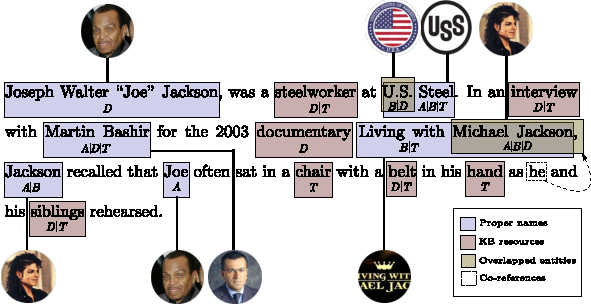
\includegraphics[width=1\textwidth]{figs/fig_annotation_example1}
\caption{Examples of annotations agreement for the EL systems: AIDA (\textit{A}), Babelfy (\textit{B}), DBpedia Spotlight (\textit{D}) and TAGME (\textit{T}). }
\end{figure}

This problem is solved in the specific-domain EL, where it is known in advance the set of entities that should be taken into account in the annotation process. However, in open-domain scenarios, the lack of a formal definition of which entities should be identified constitutes a challenging issue. In this paper, we center our attention in open-domain scenarios. Here, we stress the importance of formalizing a named entity definition in consensus by the EL community and how this phenomenon can affect the decision in the annotation process.


\section{What is named entity?}

One of the first efforts to recognize the importance of entities is coined to the $6^{th}$ Message Understanding Conference~\cite{MUC6} (MUC-6), where the concept of \textit{named entity} was defined as those terms that refer to instances of proper-name classes such as person, location and organization, and also, to numerical classes as temporal expressions and quantities. 


Despite the progress made dealing with named entities, there is not consensus about the definition of an entity in the community~\cite{Borrega007,Ling2015}. Some authors defend the proposal of MUC-6, incorporating new classes into the initial definition such as products, financial~\cite{meantime16}, film, scientist~\cite{Etzioni05} and others. On the other hand, Fleischman~\cite{Fleischman001} proposes to separate the classes into multiple specific subclasses (e.g., city, state, country from the class location). More general definitions have been used but lack of formality\cite{Eckhardt14,Uren06} (e.g., ``\textit{substrings corresponding to world entities}"~\cite{Ling2015}). Opposite, a more specific point of view is handled by Perera et al.~\cite{Perera16}, which refer to the concept of entity as those Wikipedia pages that have no ambiguity.

%%----------------


%este parrafo debería ir abajo
%It is reasonable that there are several golds standards in conflict due to the absence of a formal definition of named entities. In fact, we do not how to assess the absence/presence of basic concepts commonly found in text documents. 


\section{Issues in Entity Linking}

%Proper name
The fact of not having a consensus of entity definition accepted by the EL community brings with it other disadvantages. First of all, we do not know if the current EL systems are selecting the entities correctly. Having more than one entity definition makes the process of identifying which entities annotate ambiguously. Many authors follow the proposition of MUC-6 and separate the entities in types~\cite{meantime16,Fleischman001} to cover all the proper names, including some numerical expressions. In Figure \ref{fig:example} the proper names were mostly annotated, however, none of the systems annotate the mention of the year 2003, belonging to the group \textit{Timex} of MUC-6. Separating the entities by their type provides a structure among the entities that allows a more specific analysis and process. On the other hand, there are a plethora of entity types defined simultaneously without consensus on what should be used in the EL community.

%KB resources
The aforementioned entity assumption of Perera et al.~\cite{Perera16}, is wide used. In Figure \ref{fig:example} we can see that some system recognize nouns that have a respective knowledge base resource, but in those cases the entity refers to general concepts and not specific real-life objects. While DBpedia Spotlight and Tagme annotate \textit{belt} in Figure \ref{fig:example}, AIDA and Babelfy do not. These types of entities are valuable in the context of semantic annotation, where each concept must be identified and associated with a \textit{subject-predicate-object} rule. 

%Overlapped entities
%Bettina Fazzinga. Semantic search on the Web
Some discordances rely also on the EL definition. It is commonly accepted to identify  consecutive sequences of words in a text document, but some authors considerate instead overlapping fragments of the text~\cite{Babelfy14,Luo2015}. In this way, the entity identified in the text can overlap words each other, and as consequence, the difficulty of the EL process increases. For Instance, we can see in Figure \ref{fig:example} that Babelfy recognize ``Living with Michael Jackson" and also just the fraction ``Michael Jackson" at the same time, as well as ``U.S. Steel" and ``U.S.". Another overlap suggested by Tagme in this example is ``Living with Michael Jackson" and the wrong annotation ``Jackson, Jackson" referencing to an Australian hip hop group with this name. Depending on the application, overlapped entities can be desirables or not. In the case of the semantic web search, an adoption of overlapping entities would be appropriate in order to identify a greater number of key entities in the web page, and in this way, ``Michael Jackson" could be identified from ``Living with Michael Jackson" in a context related to him. On the other hand, Jha et al.~\cite{Jha2017}, propose to obviate overlapping entities taking into account only the larger entity.



%co-references
Other confused phenomenon in EL is the co-references, i.e., the linguistic expressions or entity mention that refer to the same entity. Although this process is implicit for proper names when it establishes the same annotation for different occurrences of the same entity in the text (e.g., ``Joseph Walter `Joe' Jackson" and ``Joe"), there is no consensus on what to do by linguistic expressions such as pronouns (e.g., in Figure \ref{fig:example} ``he" refers to ``Michael Jackson"). While Jha et al. propose leaving aside this kind of annotation to other areas such as the resolution of co-reference, other authors argue that annotate co-reference help to solve ambiguous cases of semantic types~\cite{Durrett2014}. The linguistic expressions in EL can favor particular scenarios, for example, in the semantic web search task, where the number of occurrences per entity is relevant.


\begin{table}[tbh!]
\centering
\caption{Dataset features. (Abbreviations: \textit{Ovr} denotes the presence of overlap, \textit{Cor} denotes the presence of co-references, \textit{Typ} indicates that the annotations have information about the type of the entities, \textit{PoS} indicate that have the grammatical annotation.)}
\label{tab:golds}
\begin{tabular}{lcccc}
\toprule
\textbf{System}~~~~~~~~~~~~~~~~~~~~~ &~~~\textbf{Ovr}~~~ &~~~\textbf{Cor}~~~ &~~~\textbf{Typ}~~~ &~~~\textbf{PoS}~~~ \\ \midrule
AIDA/CoNLL                    &\xmark  &\xmark &\cmark &\cmark\\
KORE50                        &\xmark  &\xmark &\xmark &\xmark\\ 
IITB                          &\xmark  &\xmark &\xmark &\xmark\\ 
OKE challenge 2016            &\xmark  &\cmark &\xmark &\xmark\\
MSNBC                         &\xmark  &\xmark &\xmark &\xmark\\
MEANTIME \cite{meantime16}    &\xmark  &\cmark &\cmark &\cmark\\ 
DBpedia Spotlight \cite{Mendes2011DBpediaSpotligth}
                              &\xmark  &\xmark &\xmark &\xmark\\
WSDM                          &\xmark  &\xmark &\xmark &\xmark\\
SenEval 2015 Task 13          &\cmark  &\xmark &\xmark &\cmark\\
N3-RSS 500                    &\xmark  &\xmark &\xmark &\xmark\\
Derczynski                    &\xmark  &\xmark &\cmark &\cmark\\
ACE2004                       &\xmark  &\xmark &\xmark &\xmark\\
\bottomrule
\end{tabular}
\end{table}

This lack of consensus means that other aspects of EL are affected, among them, we are not sure if we obtain reliable results in our evaluations process, because the correctness of the current gold standards is in doubt. A recent study of Jha et al. evidence this problem, and propose a checking tool to validate EL gold standards as well as a set of reasonable rules to stress good practices for benchmark creation. These rules constitute a forward step in order to achieve more reliable results and evidence the need to establish guidelines for the creation of gold standards.



In Table~\ref{tab:golds}, we show an overview of the most popular gold standards and their absence/presence of the aforementioned features. We can see that these gold standards are very different from each other, which leaves open the idea of standardizing their process of creation and usage. Involve high-quality gold standards provide in benchmarks the possibility of obtaining more reliable results. A more recent trend has emerged to achieve multilingual EL systems, as well as a multilingual benchmarks, which inherit the proposed disadvantages for traditional EL. See~\cite{LD4IE2017} for an overview of multilingual EL approaches.




\section{Conclusion}
\label{sec:conclusion}

Nowadays, there are many definitions of an entity in the literature which has the consequence that for the same entry there are several possible annotations that comply with the proposed definitions. In this paper, we discuss how the lack of consensus regarding the entity definition affects several EL processes, among them, the entity recognition and the evaluation. 

%
%We stress in this paper some challenges and open issues relaying in EL. We evidence the need for formal definitions for the named entity concept and how this can affect many stages in EL process. In addition, other phenomena related to EL are used in a different manner in the community. Among them, the usage or not of co-reference and overlapped entities. In addition, a well definition of entity types and gold standard format is missing.

%Despite the popularity of some quality measures to evaluate the EL annotations, we highlight some drawbacks of these measures related to areas that also affect their good performance in the evaluation of EL annotations. For this reason, a more deep analysis of meta-evaluation and strong quality measures are required.


{\footnotesize
\paragraph{Acknowledgements} The work of Henry Rosales-M\'endez was supported by CONICYT-PCHA/Doctorado Nacional/2016-21160017. The work was also supported by the Millennium Nucleus Center for Semantic Web Research under Grant NC120004.}


\bibliographystyle{splncs}
\begin{thebibliography}{99}

\bibitem{Borrega007} 
Borrega, O., Taul\'e, M., Mart\'i, M.A. What do we mean when we speak about Named Entities. In Proceedings of Corpus Linguistics, 2007

\bibitem{Ling2015}
Ling, X., Singh, S., Weld, D. S. Design challenges for entity linking. TACL \textbf{3} (2015) 315--328

\bibitem{MUC6}
Grishman, R., and Sundheim, B. Message understanding conference-6: A brief history. In COLING \textbf{1} (1996)

\bibitem{Eckhardt14}
Eckhardt, A., Hre\v{s}ko, J., Proch\'azka, J., Smr\'i, O. Entity linking based on the co-occurrence graph and entity probability. ERD, ACM (2014) 37--44

\bibitem{Uren06}
Uren, V., Cimiano, P., Iria, J., Handschuh, S., Vargas-Vera, M., Motta, E., Ciravegna, F. Semantic annotation for knowledge management: Requirements and a survey of the state of the art. Journal of Web Semantics, \textbf{4}(1) (2006) 14--28

\bibitem{Perera16}
Perera, S., Mendes, P. N., Alex, A., Sheth, A. P., Thirunarayan, K. Implicit entity linking in tweets. In ISWC, (2016) 118--132

\bibitem{meantime16}
Minard, A. L., Speranza, M., Urizar, R., Altuna, B., van Erp, M. G. J., Schoen, A. M., van Son, C. M. MEANTIME, the NewsReader multilingual event and time corpus. LREC-ELRA (2016)

\bibitem{Etzioni05}
Etzioni, O., Cafarella, M., Downey, D., Popescu, A. M., Shaked, T., Soderland, S., Daniel S. W., Yates, A. Unsupervised named-entity extraction from the web: An experimental study. Artificial intelligence, \textbf{165}(1) (2005) 91--134

\bibitem{Fleischman001}
Fleischman, M. Automated subcategorization of named entities. In ACL (2001) 25--30

\bibitem{Babelfy14}
Moro, A., Raganato, A.,  Navigli, R. Entity linking meets word sense disambiguation: a unified approach. TACL \textbf{2} (2014) 231--244

\bibitem{Luo2015}
Luo, G., Huang, X., Lin, C. Y., Nie, Z. Joint entity recognition and disambiguation. In EMNLP (2015) 879--888


\bibitem{Zheng15}
Zheng, J. G., Howsmon, D., Zhang, B., Hahn, J., McGuinness, D., Hendler, J., and Ji, H. Entity linking for biomedical literature. BMC Med Inform Decis Mak \textbf{15}(1) (2015) S4

\bibitem{Basile15}
Basile, P., Basile, V., Nissim, M., Novielli, N. Deep tweets: from entity linking to sentiment analysis. In CLiC-it (2015)

\bibitem{Song2017}
Song, H., Ren, Z., Liang, S., Li, P., Ma, J., de Rijke, M. Summarizing answers in non-factoid community question-answering. In Proceedings of the Tenth ACM International Conference on Web Search and Data Mining, ACM (2017) 405--414

\bibitem{Yih15}
Yih, S. W. T., Chang, M. W., He, X., Gao, J. Semantic parsing via staged query graph generation: Question answering with knowledge base, ACL-IJCNLP, \textbf{1} (2015) 1321--1331 

\bibitem{Jha2017}
Jha, K., R\"oder, M., Ngomo, A. C. N. All that glitters is not gold–rule-based curation of reference datasets for named entity recognition and entity linking. In ESWC (2017) 305--320

\bibitem{Ferragina10}
Ferragina, P., Scaiella, U. Tagme: on-the-fly annotation of short text fragments (by wikipedia entities). In CIKM (2010) 1625--1628

\bibitem{Mendes2011DBpediaSpotligth}
Mendes, P. N., Jakob, M., García-Silva, A., Bizer, C. DBpedia spotlight: shedding light on the web of documents. In I-Semantics (2011) 1--8

\bibitem{usbeck2014agdistis}
Usbeck, R., Ngomo, A. C. N., R\"oder, M., Gerber, D., Coelho, S. A., Auer, S., Both, A. AGDISTIS-graph-based disambiguation of named entities using linked data. In ISWC (2014) 457--471

\bibitem{Durrett2014}
Durrett, G., Klein, D. A joint model for entity analysis: Coreference, typing, and linking. TACL \textbf{2} (2014) 477--490

\bibitem{LD4IE2017}
Rosales-M\'endez, H., Poblete, B., Hogan, A. Multilingual Entity Linking: Comparing English and Spanish. In LD4IE (2017)

\end{thebibliography}

\end{document}
